
\section{De Haas-van Alphen torque measurement}

In this section the measurement of \ac{dHvA} oscillations by the torque method is described. For decades, the measurement of \ac{dHvA} oscillations provided the principle method of characterising the Fermiology of a material with only relatively recent competition from techniques such as positron annihilation and \ac{ARPES} in particular. Whilst \ac{ARPES} can provide direct maps of Fermi surfaces within the \ac{BZ}, \ac{dHvA} has some advantages such as the fact that it is insensitive to surface effects such as crystal reconstruction, can determine cross-sectional areas with a relatively high resolution and also provides useful secondary measurements such as effective masses of the quasiparticle carriers.  Some disadvantages of the technique include the fact that \ac{dHvA} cannot locate particular cross-sectional orbits within the \ac{BZ} (thus relies on secondary knowledge such as \ac{DFT} calculations) and also that the high magnetic fields could potentially affect the Fermi surface, for example by splitting the energy levels. Regardless \ac{dHvA} continues to be a reliable technique for Fermi surface characterisation.

\subsection{Experimental apparatus}

Much of the experiment apparatus has already been described in great detail by Dr. C. Andrew in her thesis~\cite{Andrew2010}. Here we recap and also detail the points of difference. 
%Moreover, although important experimental parameters will be specified, full details of the configuration of the hardware is listed in appendix~\ref{Appendix:dHvAHardwareSetup}.

\subsubsection{Torque cantilever}

A highly sensitive measure of torque is required to pick up the moments experienced by the sample due to the field. For this reason a commercial piezoelectric \ac{AFM} cantilever, provided by Seiko corps., was repurposed to measure this. The sample was placed onto the topside of the lever above the \ac{AFM} tip. Previously this would be epoxied in place but for these measurements we tried successfully with using vacuum grease which freezes the sample in place at low temperatures. This has the added benefit of still being adjustable and removable when warmed back to room temperature. Moreover, when it comes to rotate the sample in the basal plane, this was possible by nudging the sample gently without having to move the cantilever and risk breaking the lever with the sample permanently affixed. Care should be taken not to get grease on the pivot point of the levers since this will freeze the lever in place at low temperatures.
\begin{figure}[htbp]
    \begin{center}
        \includegraphics[scale=1.1]{Chapter-ExperimentalTechnique/Figures/CantileverSchematic/CantileverSchematic}
        \caption{Photo of the \BaFeP sample mounted on the measurement lever along with a schematic showing the full cantilever assembly. N.b. the \BaFeP crystals often cleave along the $[110]$ plane and so despite the apparent $45^\circ$ rotation, the sample is aligned such that the lever flexes in the $[100]$ plane.}
        \label{Fig:Exp:CantileverSchematic}
    \end{center}
\end{figure}
The cantilevers feature a second dummy lever alongside the principle lever where the sample was mounted. Instead of measuring the voltage across the principle lever alone, we measure the difference of the voltages between the two levers using a Wheatstone bridge which is balanced using two \unit{500}{\ohm} resistors. This enables some degree of correction due to vibrations and fluctuations in measurement current and also allow for correction of magnetoresistance effects within the levers. The circuit is balanced using a variable resistor and is zeroed as best as possible within the noise before each measurement run.

The voltage is supplied and measured using Stanford SR830 lock-in amplifier. The input supplied to the Wheatstone bridge first passes through a \unit{10}{\kilo\ohm} resistor with an excitation voltage of \unit{1}{\volt} unless otherwise stated. The output is first amplified using an EG\&G 5113 pre-amplifier with a gain of $\times1000$ with a band pass filter which was suitably set for the lock-in amplifier excitation frequency. All of the circuitry mentioned above, aside from the cantilevers and leads, is kept outside of the fridge at room temperature and is away from the field centre by approximately \unit{2-3}{\metre}.

\subsubsection{Sample stage}

The cantilever is mounted onto the sample stage which is a one axis Swedish rotator fabricated entirely from hysol. This is moved by an external stepper motor controlled by a computer. 

The angle of the stage in relation to the field is determined by one of two orthogonal pick-up coils mounted on the sample stage. A weak, oscillating magnetic field is generated by a coil which is wound concentrically around the inside of the main magnet coil. The AC coil induces a voltage in these orthogonal pick-up coils on the stage which is proportional to the sine of the angle they are at with respect to the field. The pick-up coil voltage is measured by a second Stanford SR830 lock-in amplifier after passing through a custom amplifier set to $\times100$. The lock-in amplifier also drives the oscillating field after passing a custom built current source. The modulating coil is designed to generate an oscillating field of a few tens of Gauss whilst the main coil is in persistent mode~\cite{Instruments1998}.

% An upper bound on the strength is $\sim$\unit{333}{\textrm{Gauss}} RMS, based on a typical measured voltage of \unit{2.2}{\milli\volt} after $\times100$ amplification measured across a coil of $\sim140$ turns with an average area of \unit{3.36}{\milli\metre\squared} per loop.

\subsubsection{Yellow Magnet}

Measurements of the oscillations were all performed in Bristol on the `Yellow Magnet' system which was built by Oxford and can nominally operate up to \unit{20.5}{\tesla} with use of the lambda plate, an additional cooling system for the magnet coil, although is more typically operated up to \unit{18}{\tesla}.
\begin{figure}[htbp]
    \begin{center}
        \includegraphics[scale=1.1]{Chapter-ExperimentalTechnique/Figures/SampleStageSchematic/SampleStageSchematic}
        \caption{A photo of the Swedish rotator sample stage with cantilever in place and protective cap removed.}
        \label{Fig:Exp:SampleStageSchematic}
    \end{center}
\end{figure}
The bulk of the cryostat sits in a bath of $^4$He which takes the temperature down to the helium boiling point of \unit{4.2}{\kelvin}, and then the sealed sample space is additionally immersed in $^3$He gas in a Heliox system. This system condenses the $^3$He gas at the base of the chamber and pumps on it using a charcoal sorb to lower the sample stage temperature to $\sim$\unit{0.3}{\kelvin} for several hours before it has to be re condensed. Figure~\ref{Fig:Exp:YellowFridge} demonstrates the condensing cycle.
\begin{figure}[htbp]
    \begin{center}
        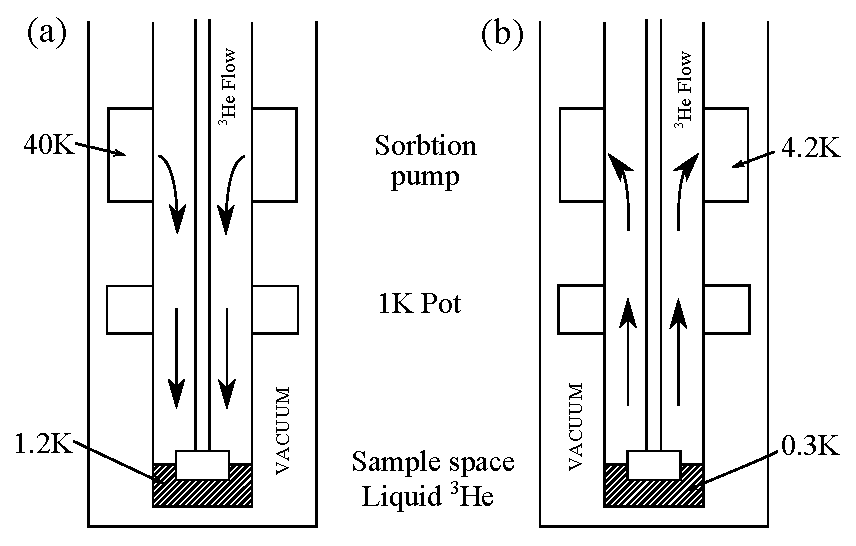
\includegraphics[scale=0.6]{Chapter-ExperimentalTechnique/Figures/YellowFridge/YellowFridge}
        \caption{The $^3$He condensing cycle for the Yellow Magnet Heliox. (a) The sorbtion pump is heated so the $^3$He it contains is released and condenses into a fluid on reaching the \unit{1}{\kelvin} pot. (b) Once a significant proportion of the $^3$He is condensed, then the pump heater is switched off which pumps on the liquid causing additional cooling around th esampel stage to $\sim\unit{0.3}{\kelvin}$}.
        \label{Fig:Exp:YellowFridge}
    \end{center}
\end{figure}
 In general measurements are taken at base temperature but higher temperatures can be achieved by heating the charcoal sorb pump thus lowering the pumping rate on the $^3$He bath. This technique allows access to temperatures up to approximately \unit{2.1}{\kelvin}. Temperatures greater than this are possible by heating the sample through an electric heater mounted on the magnet, however with our setup we do not accurately control temperature as the field ramps because of complications due to magnetoresistance effects in the measurement thermometers. Temperature is monitored at the sample by a Cernox thermometer on the sample stage, and a RuO$_2$ thermometer which is mounted in the sample space on the cryostat but is in thermal contact with the tip of the sample stage when the stage is properly seated. Care should be taken that this is the case to ensure effective pre-cooling of the sample. Further thermometers are situated on the \unit{1}{\kelvin} pot, the sorb and sat on top of the magnet coil although the latter is only monitored when initially cooling the magnet from room temperature. All thermometers and heaters were controlled using two Neocera LTC-21 temperature controllers.

Data is collected by a Windows PC running custom Delphi software which queues measurements and records data only. No analysis is performed in the collection software. Data is saved to text files.

\subsection{Data analysis}

\subsubsection{Angle correction}
    \label{Sec:Exp:AngleCorrection}

To perform angle dependent measurements, we need to first of all measure accurately the angle between subsequent measurements and second we need to determine the angle of the field compared to the basal planes of the crystal. 

In order to tackle the first problem, the pick-up coils sampling the AC field described earlier are used with the measured voltage begin proportional to the sine of the angle between the coil and the AC field. By monitoring this voltage, accurate determination of the angle between the sample platform and the field can be made and therefore the angle between subsequent measurements.

The absolute angle between the large DC field and the crystal planes in the sample were determined using a post-measurement correction. Since the frequency of the quantum oscillations are field dependent with turning points at the $B\parallel [001]$ direction for approximately two dimensional samples, an even termed polynomial up to fourth order was fitted to the peaks. From the minima of the fits an angular offset was obtained which gave the final correction to the above coil measurements.

The basal angle was aligned on the cantilever by eye. This was coupled with \ac{XRD} measurements which determined how the visual features corresponded to the crystal axes. This leads to an estimated error in basal plane alignment of around \unit{5}{\%} although we found evidence for greater misalignment in one case, detailed in the results.

\subsubsection{Temperature correction}
    \label{Sec:Exp:TemperatureCorrection}

Effective mass measurements on particular extremal orbits rely on accurate temperature determination at all stages of the field sweep. On the Yellow magnet system, temperature from base of $\sim$\unit{0.3}{\kelvin} to $\sim$\unit{2}{\kelvin} is controlled by adjusting the $^3$He sorbtion pump temperature and is largely independent of field effect since the thermometer regulating the sorb temperature is outside of the strong field core. However if we consider figure~\ref{Fig:Exp:TemperatureCorrection}, it is evident that there are magnetic field effects on the RuO$_2$, which is mounted in the base of the magnet but thermally linked with the sample, and the Cernox thermometer that sits on the sample stage.
\begin{figure}[htbp]
    \begin{center}
        \includegraphics[scale=0.9]{Chapter-ExperimentalTechnique/Figures/TemperatureCorrection/TemperatureCorrection}
        \caption{Some example temperature readings (filled symbols) set using the sorbtion pump heater. Also shown are corrections (open symbols) by interpolating to known values. RuO$_2$ thermometer is shown as circles, Cernox stage thermometer is shown as squares. Second order polynomial fits to the data are shown as lines extrapolated to zero to get a rough estimate of the zero field temperature value.}
        \label{Fig:Exp:TemperatureCorrection}
    \end{center}
\end{figure}
Readings from both thermometers were taken with field sweeps from zero field up to \unit{18}{\tesla} at steady temperatures \unit{0.30}{\kelvin}, \unit{0.53}{\kelvin}, \unit{0.64}{\kelvin}, \unit{1.06}{\kelvin} and \unit{1.34}{\kelvin}. By interpolating between this data\footnote{Performed using multiquadric radial basis functions from the Scipy Python library.}, the two thermometers can be corrected to agree within $\sim$\unit{0.01}{\kelvin}. This interpolation is however limited to temperatures below approximately \unit{1.45}{\kelvin} as is shown in the figure for readings at around \unit{1.6}{\kelvin}. In these cases, the less reliable method of extrapolating the readings back to zero field using a second order polynomial fit are used as demonstrated with the solid lines in figure~\ref{Fig:Exp:TemperatureCorrection}. In these cases the temperature is taken to be the mean of the two extrapolated values with the differences defining the error.

\subsubsection{Self heating effects}

The resistance across the piezo-electric lever is read by driving an AC current through it and reading the voltage across it using the Stanford lock-in amplifier. Larger currents are less prone to noise problems, however too much current results in self heating and subsequently the sample platform and sample could be at a higher temperature than the nearby thermometers suggest. To ensure that this is not the case we measure oscillations at constant temperature with a variety of driving currents. Small currents should not affect oscillation amplitudes, but at some current threshold self heating effects will become apparent and the oscillations are damped as if the entire system was operating at a higher temperature. We then resume measurements using a driving current below this threshold.

Ideally the temperature chosen should be on the steep part of the \ac{LK} temperature curve (eq.~\ref{Eqn:Theo:TemperatureTerm}) so that even small changes in temperature manifest in observable changes in the oscillation amplitude.

% \subsubsection{Field hysteresis correction}
% 
% Although the direction in which the field sweep occurs should not affect the oscillations, it was apparent that there was a slight shifting of the \ac{FFT} frequencies of the peaks in the down sweeps in comparison to the upsweeps. The shifts were larger at higher frequencies and generally would be of the order of \unit{0-40}{\tesla}. Since the effect was clear yet was of the order of the expected reolution at high fields, we simply applied a linear correction to the data set in order to bring the peaks into line. The corrections listed in table~\ref{Table:Exp:HysteresisCorrection} were either subtracted or added depending on the sweep direction.
% \begin{table}
%     \begin{center}
%            \caption{Correction factors linearly applied to the \ac{FFT} peaks due to hysteresis in the sweep direction.}
%         \begin{tabular}[htbp]{lll}
% \toprule
% Sweeps $B \to[110]$ & Corrn. at \unit{0}{\tesla}  & Corrn. at \unit{8000}{\tesla}\\
% \midrule
% $-31\degree$ to $-24\degree$  & 1 & 18 \\
% $-24\degree$ to $-13\degree$ & 9 & 20 \\
% $-13\degree$ to $100\degree$ & 1 & 21 \\
% \bottomrule
% & & \\
% \toprule
% Sweeps $B \to[100]$ & Corrn. at \unit{0}{\tesla}  & Corrn. at \unit{8000}{\tesla}\\
% \midrule
% $-31\degree$ to $100\degree$ & 3 & 13 \\
% \bottomrule
%         \label{Table:Exp:HysteresisCorrection}
%         \end{tabular}
%     \end{center}
% \end{table}

\subsubsection{Torque measurement factor}

An extra factor affecting the amplitude of the \ac{LK} oscillations occurs due solely to the nature of the torque oscillation measurement. The factor is given by,
\begin{equation}
    A_{\Gamma \textrm{(gen)}} = \frac{1}{F}\frac{dF}{d\theta_\perp}B
\end{equation}
where $\theta_\perp$ is the angle from the field direction. This can be simplified for a quasi $2d$ metal to,
\begin{equation}
    A_{\Gamma} = |\sin(\theta)|B
\end{equation}
where $\theta$ is the angle from the cylinder axis (usually in the $c$ direction). This means that at along the cylinder axis there will be no oscillations as $A_{\Gamma} \to 0$.


\subsubsection{Background removal}

Previous standard practice was to remove a background polynomial fitted to the field or inverse field from the raw data before taking the \ac{FFT}. With reference to figure~\ref{Fig:Exp:RawPlotAngleDependence}, raw torque data taken over a range of angles\footnote{See section\ref{Sec:ResD:AngleDependentMeasurements} for full details} and a strong $B^2$ component can be observed as a result of the $A_{\Gamma}$ term in the \ac{LK} equation at angles away from \unit{90}{\degree} and \unit{0}{\degree}. Figure~\ref{Fig:Exp:BackgroundSubtraction} shows in the centre and right panels that subtracting a second order polynomial fitted to the \emph{inverse} field leaves a large artificial angle-dependant oscillation in $1/B$ in the residual which may be misconstrued as a signal from a low frequency Fermi surface orbit, especially since there is an apparent angle dependence -- no such peak is seen for the flat curves at \unit{0}{\degree} and \unit{90}{\degree}. For this reason it is recommended to subtract a second order polynomial fitted to field rather than inverse field for torque measurements.
\begin{figure}[htbp]
    \begin{center}
        \includegraphics[scale=1.1]{Chapter-ExperimentalTechnique/Figures/ComparisonBackgroundSubtraction/RawPlotAngleDependence}
        \caption{The angle dependence of the raw torque data clearly showing a negative $B^2$ background at \unit{45}{\degree} and for $\theta<\unit{90}{\degree}$ and a positive $B^2$ background for $\theta>\unit{90}{\degree}$.}
        \label{Fig:Exp:RawPlotAngleDependence}
    \end{center}
\end{figure}
\begin{figure}[h!]
    \begin{center}
        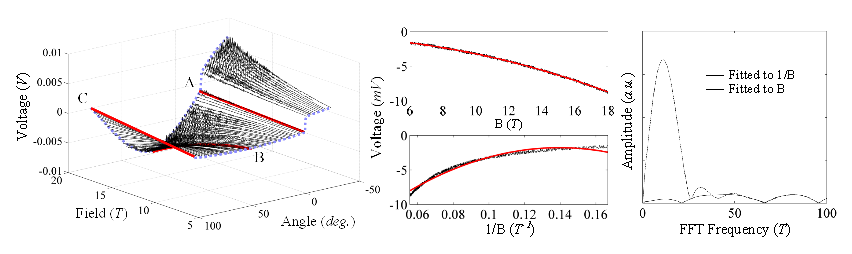
\includegraphics[scale=1.1]{Chapter-ExperimentalTechnique/Figures/ComparisonBackgroundSubtraction/ComparisonBackgroundSubtraction}
        \caption{Insets show a 2nd order polynomials fitted to simulated $B^2$ background with $\sim$\unit{0.5}{\milli\volt} of noise, similar in scale to that of \unit{45}{\degree} in figure~\ref{Fig:Exp:RawPlotAngleDependence}. Upper inset is fitted to field and lower to inverse field. The main figure shows the resulting \acp{FFT}.}
        \label{Fig:Exp:BackgroundSubtraction}
    \end{center}
\end{figure}

\subsection{Measuring the spin mass}
\label{Sec:Exp:MeasuringSpinMass}

Other than beating effect from similar frequencies, the only terms in the \ac{LK} equation that cause the amplitude to drop to zero as a function of angle are the torque term, $A_\Gamma$ which causes a single zero when the field is parallel with the cantilever arm and the spin term $A_S$\footnote{The angle dependence of $A_S$ comes from variations in the band mass}. By examining the amplitude as a function of angle it is possible to determine the spin effective mass. A good determination requires more than one spin zero (i.e. a non torque term zero) to be measured since the oscillatory nature of the $A_S$ term gives multiple solutions if we only have measured a single zero. We use $n$ to label each of the zeros from the $A_S$ oscillations.

% In practice the determination is complicated by the fact that if the Landau levels are very well defined, the double peaks due to Zeeman splitting do not overlap and so do not interfere. This manifests as a splitting of amplitudes which do not necessarily drop to zero. In these cases the zeros have to be best determined as being within the region where a noticeable increase in the number of spin split peaks occurs. Moreover, 

In practice, fitting the overall shape requires all of the \ac{LK} terms to be considered which makes free parameter fitting very difficult to converge. For these reasons, spin mass for this investigation is found from ansatz guesses for the values which are then fitted by inspection. Upper and lower bounds for the estimations are provided.

To the first approximation, the cylindrical approximation is used to describe the band mass in $A_S$, however the form of the spin term is relatively sensitive to small deviations and so fits would be much better using a more accurate variation of band mass with angle. Band mass was extracted from \ac{DFT} results and was performed using MATLAB code which locates the extremal areas from the corrected \ac{BZ} energy dispersion at a particular angle. Once located a small shift in energy is applied and the corresponding shift in area is used to determine the band mass using equation~\ref{Eqn:Theo:BandMass}. A polynomial of appropriate order is then fitted to the curve and used in the fitting routine in place of the band mass. The MATLAB code determines the masses with some spread in the values which caused higher order polynomial fits to oscillate at low angles within the noise. To alleviate this, a mean value was determined for each angle.

One final note is that the absolute value of the $A_S$ term is used to fit the data since we analyse the height of the \ac{FFT} peaks of the oscillations which are always positive and not the oscillations directly.

\subsection{Extracting effective mass from the temperature dependence}
\label{Sec:Exp:ExtractingEffMassTemperatureDependence}

Of all the damping terms in the \ac{LK} equation, only $A_T$ (eqn.~\ref{Eqn:Theo:TemperatureTerm}) is temperature dependent and so is used to determine the thermal effective mass. By measuring oscillations at a fixed angle but with varying temperatures, the effective mass can be determined in a number of ways.

\subsubsection{Basic \ac{LK} formula fitting}

The simplest technique to extract the thermal effective mass is to extract the amplitude of the oscillations from \acp{FFT} of the data at various $T$ and then perform a least squares fit to eqn.~\ref{Eqn:Theo:TemperatureTerm}. A particular problem with this approach is that it is not clear what value of $B$ should be used since the \acp{FFT} needs to span a field range when ostensibly the oscillation should be measured at a particular $B$ value. Generally the simplest thing to do is to take the \acp{FFT} over a small a range as possible and then take the field to be equal to the averaged inverse field\footnote{That is $B_{\textrm{av.}}^{-1} = \frac{1}{2}(B_{\textrm{min}}^{-1} + B_{\textrm{max}}^{-1})$}. 

There are two conflicting problems with this approach. First the amplitude tends to decreases with narrowing field range meaning weak oscillations may require larger field intervals. Secondly wider field ranges mean other attenuation factors --- which are also functions of $B$ --- affect the amplitude across the field sweep. The primary problem in this case is the Dingle term which has an exponential dependence on $B$. Although the Dingle term is not temperature dependent, the exponential dependence on the Dingle factor changes the amplitude of the oscillations over the field range necessary for the \ac{FFT} which can affect the final amplitude. Nonetheless, simple \ac{LK} fits are usually the first port of call and serve as a first approximation to the final result. For this investigation though, since we found some disagreement within the data, we employed a couple of additional techniques described below to overcome this shortcoming.

\subsubsection{Retrofitting ansatz \ac{LK} formulae}
\label{Sec:Exp:LKRetrofitting}

One of the primary field-dependant contributions to the oscillation amplitude is the Dingle term scattering (equation \ref{Eqn:Theo:DingleTerm}) which has an exponential dependence with temperature. The Dingle factor, $\alpha \equiv -\pi p m_b/e\tau$, can be determined by fitting a simplified version of the \ac{LK} equation,
\begin{equation}
    \Gamma_{\textrm{sim}} =  A_D(\alpha, B) \sqrt{B} \sin{\left(\frac{2\pi F}{B} + \phi \right)}
\end{equation}
 to oscillations which have been band pass filtered to reduce the number of contributions from other extremal orbits and hence the number of necessary fitting parameters. Once we have the Dingle term and also the peak frequency for a particular orbit, simulated oscillations are generated using the same equation but including the temperature term, $A_T(m^*_T, B)$, for a range of ansatz effective thermal masses. We then fit this to the \ac{LK} equation as described in the previous section. The mass that results from the fit is different from the actual effective mass used as the \ac{LK} fit has been affected by the Dingle term contribution. When we find a simulated oscillation that outputs the same effective thermal mass as the plain \ac{LK} fit on the actual data we then take the ansatz thermal mass for that matching fit to be the corrected thermal mass.

The filtering used to originally separate out the frequencies is band pass \ac{FFT} using a Hanning window.  This is adjusted in size and roll off width according to the peak. Occasionally, the peaks are too close together to effectively filter out individually and so two or three peaks were fitted at a time using a linear combination of the simplified equation above.

The initial fits were filtered using an existing Delphi program and fits to find $\alpha$ were performed in Kaleidagraph. Ansatz fits were found using a binary search technique using a Python script.


\subsubsection{`Microfitting' the \ac{LK} formula}
\label{Sec:Exp:LKMicrofitting}

A second technique is to filter out the individual orbit frequency by again using an \ac{FFT} filter and a Hanning window, and this time fitting small sections of sine curve ($\sim 1.5$--$3$ wavelengths) directly to the filtered torque data. This gives a field dependent value for the amplitude which can then be fitted to the standard $A_T$ form for many values of $B$. The result is a plot of mass values against $B$. Theoretically, these should plateau to give a constant value for the effective thermal mass.

Calculations were performed using a Python script to filter the data, perform the `microfits' and then perform the \ac{LK} fits. The script was tested using simulated data.


